\chapter{Noosfero}
%TODO deixar claro quais são nossos pré-requisitos e por que escolhemos
%o noosfero; basear-se no estudo com a USP em 2010 e wikipedia (plataformas
%de rede social

Nesse capítulo fazemos um apanhado dos benefícios de se utilizar uma
plataforma de software livre e introduzimos a plataforma para criação de
redes sociais livres Noosfero. Escolhemos trabalhar com software livre por
entendermos que este é um integrante fundamental no ensino da ciência e 
tecnologia, estando alinhado à ideologia de livre compartilhamento de
conhecimento. Outro fator fundamental para a utilização de software livre é o
fato de não termos que nos comprometermos a assinar um termo de compromisso
comum em redes sociais proprietárias, que, em geral, possuem cláusula que dão à
empresa proprietária a propriedade intelectual em cima de todo o conteúdo
gerado nela.


\section{Software Livre}

Software expressa uma solução abstrata dos problemas computacionais.
%
O software, em um sistema computacional, é o componente que contém o
conhecimento relacionado aos problemas a que a computação se aplica.
%
Por isso, o software é algo de interesse geral, uma vez que vários aspectos
relacionados a ele ultrapassam as questões técnicas, como por exemplo:
\begin{itemize}
\item O processo de desenvolvimento do software; 
\item Os mecanismos econômicos (gerenciais, competitivos, sociais, cognitivos etc.)
que regem esse desenvolvimento e seu uso;
\item O relacionamento entre desenvolvedores, fornecedores e usuários do
        software;
\item Os aspectos éticos e legais relacionados ao software.
\end{itemize}

O que define e diferencia o software livre do que podemos denominar de
software restrito passa pelo entendimento desses quatro pontos dentro do que é
conhecido como o \emph{ecossistema do software livre}.
%
O princípio básico desse ecossistema é promover a liberdade do usuário,
sem discriminar quem tem permissão para usar um software e seus limites de uso,
baseado na colaboração e num processo de desenvolvimento aberto.
%
Software livre é aquele que permite aos usuários usá-lo, estudá-lo, modificá-lo e
redistribui-lo, em geral, sem restrições para tal e prevenindo que não sejam
impostas restrições aos futuros usuários.
%

Normalmente, esse software existe por meio de projetos de desenvolvimento
que estão centradas em torno de algum código-fonte acessível ao público,
geralmente em um repositório na Internet, onde desenvolvedores e usuários
podem interagir.
%
O código é necessariamente licenciado sob termos legais formais que estão de
acordo com as definições da \textit{Free Software Foundation}
\footnote{\url{http://www.gnu.org/philosophy/free-sw.html}} ou da
\textit{Open Source Initiative}
\footnote{\url{http://www.opensource.org/docs/definition.html}}.

%------------------------------------------------------------------------------%

Uma vantagem oferecida pelo software livre em comparação ao software
restrito vem do fato de que o código-fonte pode ser livremente compartilhado.
%
Esse compartilhamento pode simplificar o desenvolvimento de aplicações
personalizadas, que não precisam ser programadas a partir do zero, mas
podem basear-se em soluções já existentes.
%
Na medida em que o desenvolvimento de aplicações personalizadas é um dos focos do
desenvolvimento de software em geral, essa vantagem tem impacto significativo na
redução de custos e na diminuição na duplicação de esforços, tirando proveito da
característica abstrata do software.

Outra vantagem resultante do compartilhamento do código se refere
à possível melhoria na qualidade \cite{CatedralBazzar}, em particular frente aos
problemas inerentes à sua complexidade.
%
Isso se deve ao maior número de desenvolvedores e usuários envolvidos
com o software. Em outras palavras, um número maior de desenvolvedores, com diferentes
perspectivas e necessidades, é capaz de identificar melhorias e corrigir
mais \emph{bugs} em menos tempo e, consequentemente, promover refatorações que,
geralmente, levam à melhoria do código.

%
Além disso, um número maior de usuários gera situações de uso e
necessidades mais variadas, o que se traduz em um maior número
de \emph{bugs} identificados e mais sugestões de melhorias.

%------------------------------------------------------------------------------%

\section{Noosfero, Uma Plataforma Livre para Redes Sociais}
\label{noosfero-section}

Noosfero~\footnote{\url{http://www.noosfero.org}}
é uma  plataforma web livre para criação de redes sociais desenvolvida
pela Cooperativa de Tecnologias Livres - Colivre
~\footnote{\url{http://www.colivre.coop.br}} 
em 2007 sob licença AGPL v.3 com a proposta de permitir aos usuários criarem sua
própria rede social personalizada, livre e autônoma.
%
As principais funcionalidades do Noosfero incluem:

\begin{itemize}

\item Rede Social (três entidades: pessoas, comunidades e organizações);
\item CMS: pastas, artigos, RSS, \textit{upload} e publicação de imagens e
arquivos;
\item \textit{Blog} com sistema de notificação de comentários;
\item Fórum de discussões;
\item Galeria de imagens;
\item Agenda de eventos compartilhadas;
\item e-Portfolios (individuais \& de grupos);

\end{itemize}

%------------------------------------------------------------------------------%

O Noosfero foi desenvolvido na linguagem de programação Ruby
~\footnote{\url{http://www.ruby-lang.org/en/}}
versão 1.8.7 e utiliza o framework MVC para aplicações web Ruby on Rails
~\footnote{\url{http://rubyonrails.org/}}
versão 2.3.5.
%
A escolha destas tecnologias se baseou no fato de que o Ruby possui uma sintaxe
simples, elegante e de fácil leitura, o que aumenta a manutenibilidade do sistema,
uma característica importante num projeto de software livre que visa atrair
desenvolvedores externos. 
%
Outras características importantes que influenciaram essa escolha são a alta
capacidade produtiva que o framework possui por priorizar conceitos como
\textit{convention over configuration} (convenção antes de configuração)
e DRY~\footnote{Uma forma de apologia ao reuso de código}
(\textit{Don't Repeat Yourself} - Não Repita a Si Mesmo)
e o alinhamento entre a comunidade do Ruby on Rails com metodologias ágeis de
desenvolvimento de software evidenciada em uma série de ferramentas que
viabilizam o uso de práticas como TDD~\footnote{Desenvolvimento orientado a testes}
e BDD~\footnote{Design orientado a comportamento}, práticas adotadas no
desenvolvimento do Noosfero.

%------------------------------------------------------------------------------%

A segurança também foi uma preocupação na concepção do projeto, o que levou os
desenvolvedores a tomar a decisão de homologar a ferramenta apenas para a
versão do Debian~\footnote{\url{http://www.debian.org/}}
\textit{stable}, nesta fase do trabalho de acordo com a versão de codinome
\textit{Squeeze}, por este ser reconhecido por passar por rigorosos testes de
segurança e correção de falhas antes de seu lançamento. 
%
Para manter a compatibilidade, as versões do Ruby e do Rails utilizadas no
Noosfero são as versões disponibilizadas nos repositórios do Debian
\textit{Squeeze}.

%------------------------------------------------------------------------------%

A arquitetura do Noosfero foi desenvolvida para permitir que este seja facilmente
expansível, de forma que funcionalidades que não sejam comuns ao conceito de
redes sociais sejam desenvolvidos como \textit{plugins}, assim diminuindo
o acoplamento e aumentando a coesão dos diversos módulos do sistema.
%
Uma das grandes vantagens em se criar uma aplicação com arquitetura extensível
é o fato de que o desenvolvedor pode criar um \textit{plugins}
sem precisar modificar o código fonte da ferramenta, além de tornar mais
fácil o isolamento de \textit{bugs} encontrados. 

\begin{figure}[h]
	\centering
	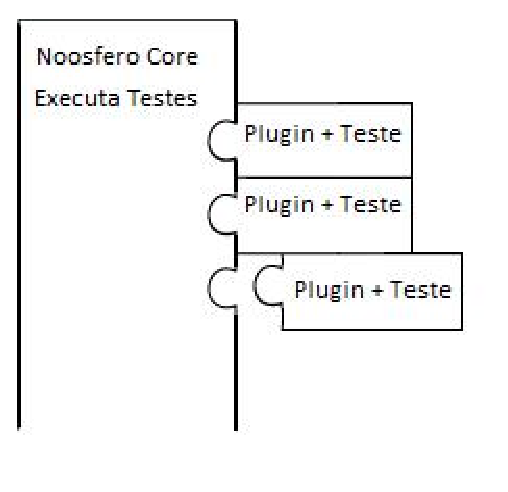
\includegraphics[keepaspectratio=true,scale=0.6]{figuras/plugins.eps}
	\caption{Arquitetura de plugins do Noosfero}
	\label{plugins}
\end{figure}

A Colivre, que atualmente é a única responsável por aprovar solicitações de
alteração no código, exige que os \textit{plugins} tenham um certo nível de
testes para que este possa ser incorporado à uma versão do Noosfero para
evitar a inserção de \textit{bugs} que afetem o \textit{core} ou
outros \textit{plugins} além de manter o padrão de qualidade de código. A
Figura \ref{plugins} apresenta a arquitetura expansível do Noosfero.

Essa abordagem arquitetural é muito benéfica para a diversidade de contextos
em que o Noosfero pode ser implantado. Diversidade esta que pode ser evidenciada
quando se observa a existência de uma rede como o Cirandas
~\footnote{\url{https://cirandas.net/}}
, uma rede social com o propósito de promover economia solidária através
da troca e venda de produtos e serviços, e o
Stoa, um ambiente virtual para a disseminação de conhecimento em âmbito
acadêmico de forma colaborativa, ambos desenvolvidos utilizando o Noosfero.
Dessa forma, os dois ambientes compartilham um núcleo comum às redes sociais
no geral, mas diferem no uso de \textit{plugins} com funcionalidades próprias
às suas necessidades específicas. Na seção \ref{requisitos}, apresentamos
algumas funcionalidades que serão desenvolvidas no formato de um \textit{plugin},
Comunidade-UnB.


%------------------------------------------------------------------------------%

A Figura \ref{noosfero-arch} apresenta uma visão arquitetural de alto nível
do núcleo do Noosfero. Vale a pena ressaltar alguns componentes desta arquitetura:

\begin{figure}[h]
	\centering
	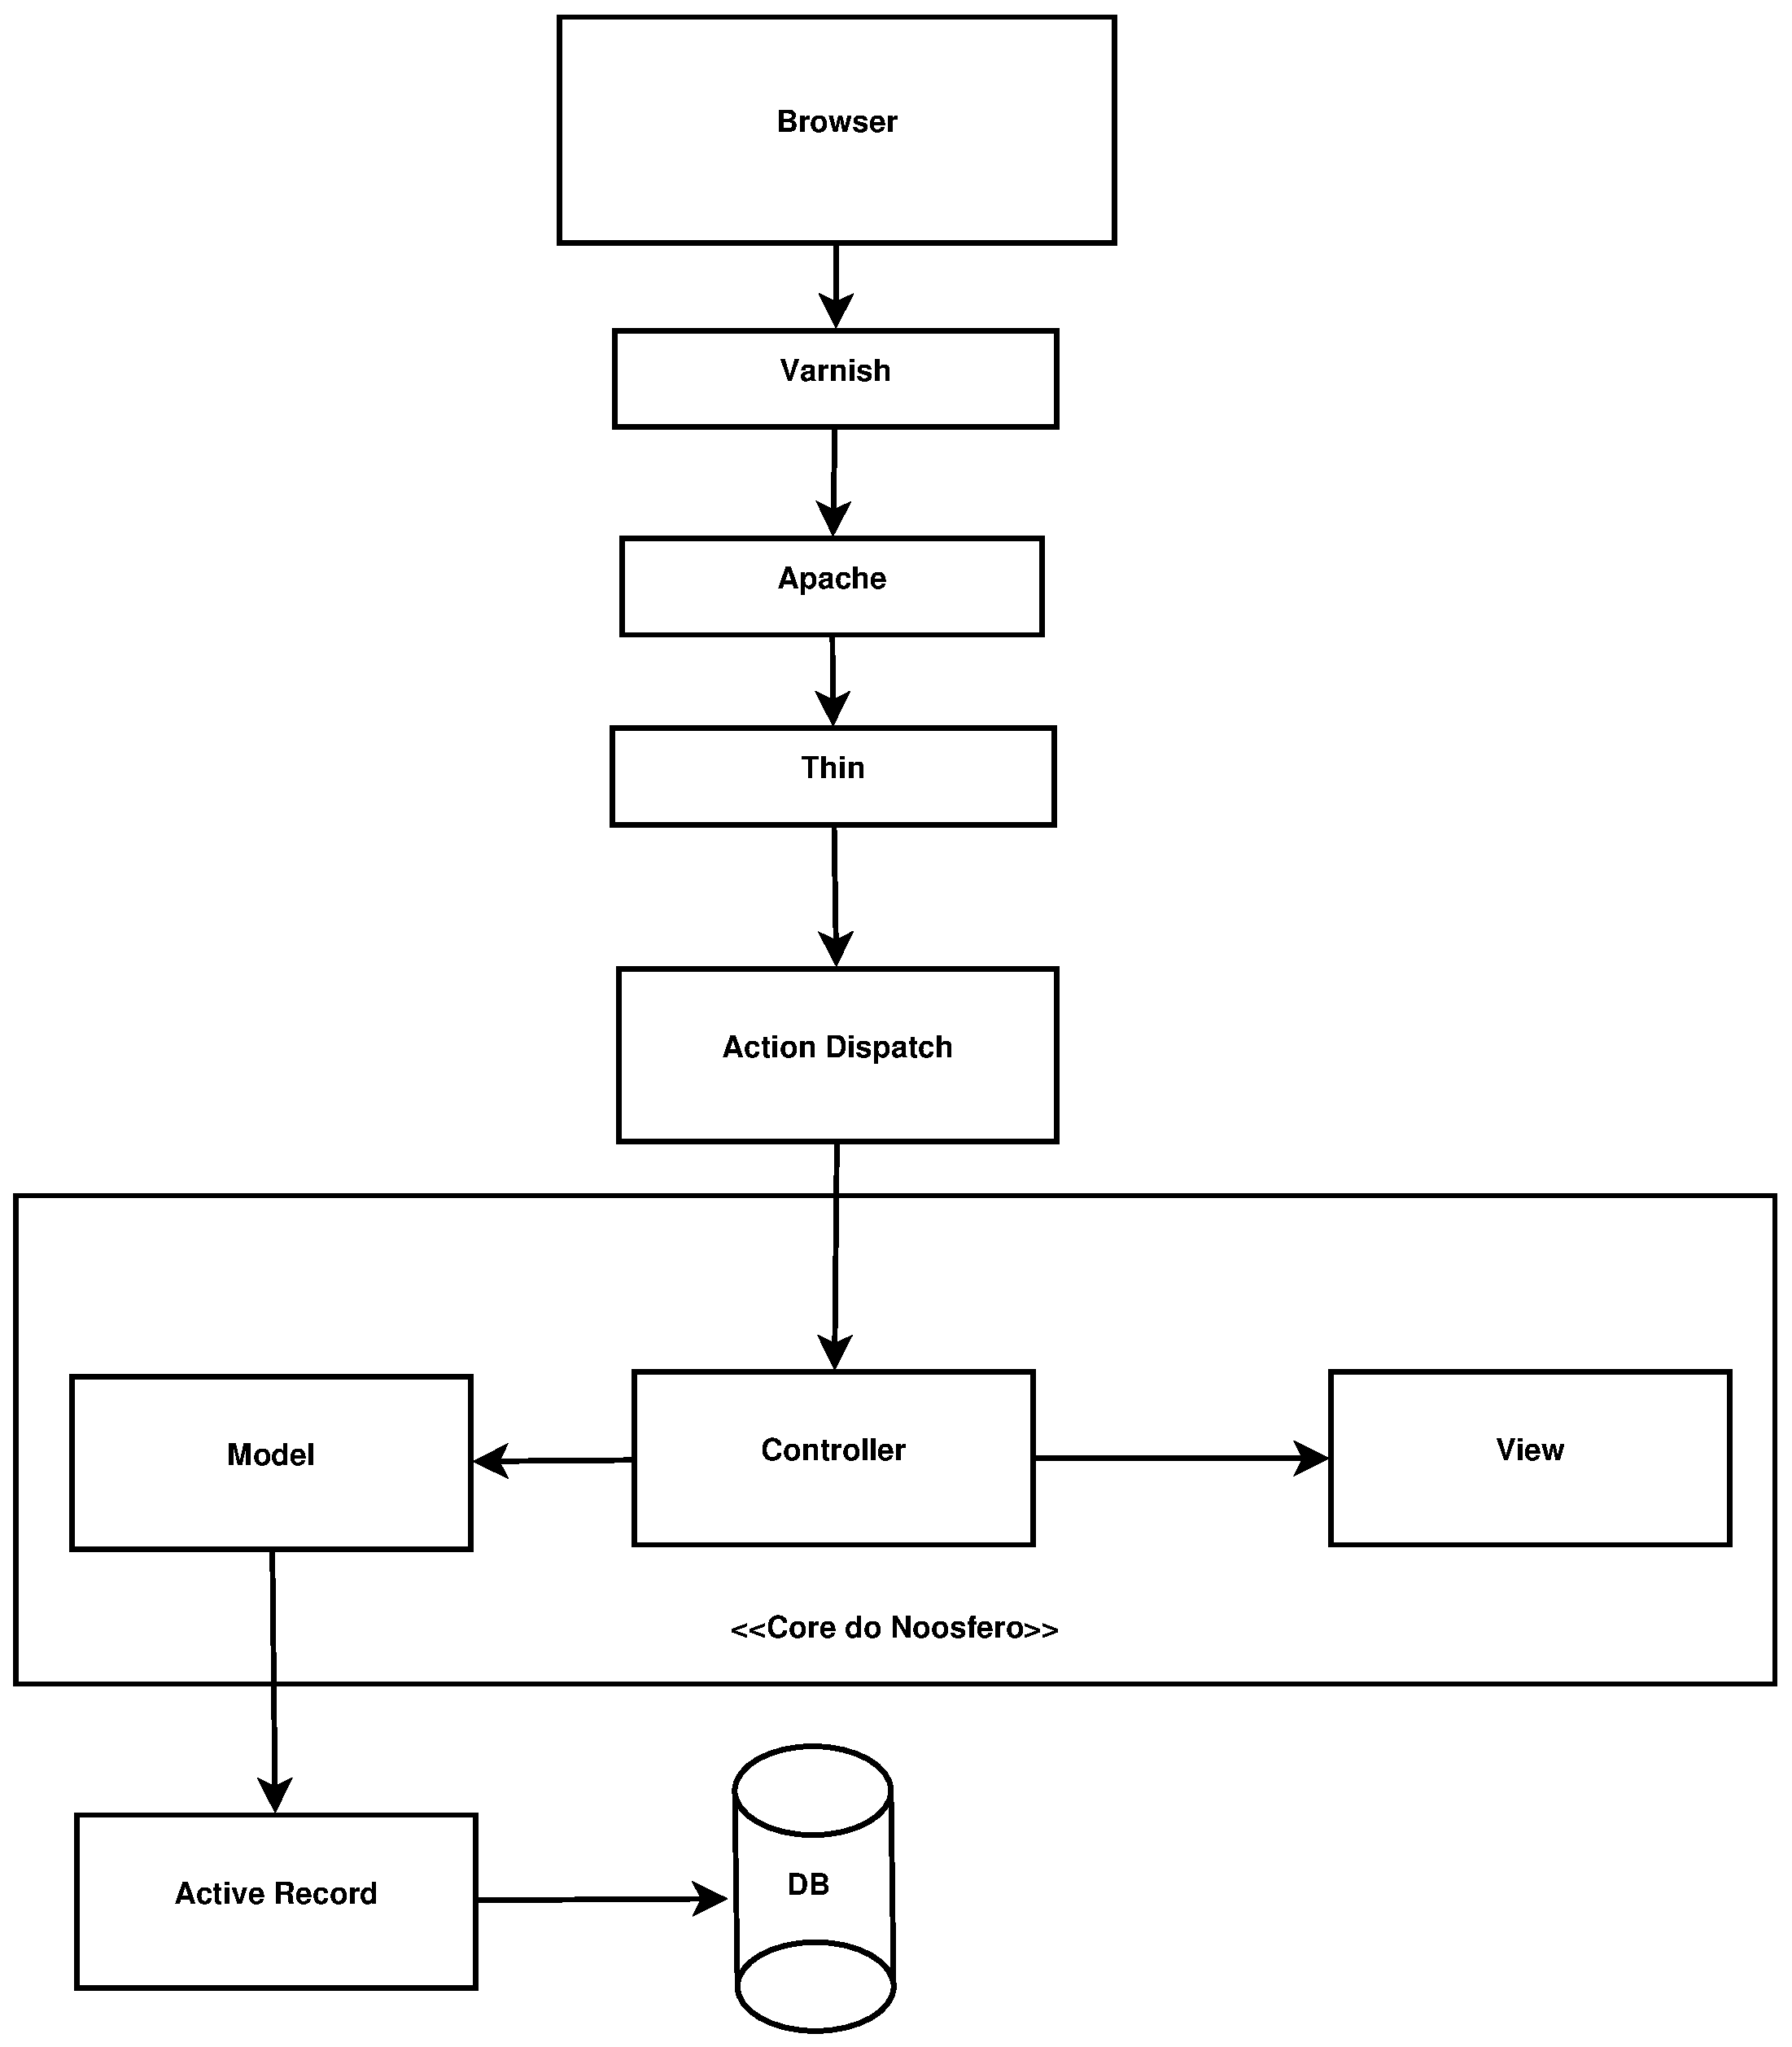
\includegraphics[keepaspectratio=true,scale=0.25]
	  {figuras/noosfero_architeture.eps}
	\caption{Visão arquitetural do Noosfero}
	\label{noosfero-arch}
\end{figure}

\begin{itemize}
	\item \textbf{Varnish:} acelerador de aplicações web também conhecido 
	como cache de proxy reverso HTTP. É utilizado quando for necessário
	acessar conteúdo estático,imagens, \textit{scripts} e folhas de estilos.

	\item \textbf{Apache:} \textit{web-server} utilizado como servidor de 
	\textit{proxy} reverso. Sua função é encaminhar as requisições que
	chegam para uma das instâncias do Thin.

	\item \textbf{Thin:} \textit{app-server} utilizado para processar as
	requisições de entrada e saída e encaminhá-las para o Noosfero para que
	este possa executá-las. Pode ser configurado para utilizar mais de um
	processo para realizar balanceamento de carga. É recomendável o uso de
	dois processos do \textit{Thin} por núcleo de processador do servidor
	hospedeiro.
	
	\item \textbf{ActionDispatch:} funciona como roteador. Sua função é
	mapear as requisições que chegam a suas respectivas \textit{controllers}.
	
	\item \textbf{Controller:} controla o fluxo da aplicação. Realiza a
	ligação entre as entidades de \textit{model} e de \textit{view} através
	de chamadas de métodos.
	
	\item \textbf{Model:} representa as entidades do domínio da aplicação.
	A lógica da aplicação é implementado nas classes de \textit{model}.

	\item \textbf{View:} responsável pela visualização das páginas, isto é,
	as saídas em HTML da aplicação.
	
	\item \textbf{Active Record:} realiza o mapeamento entre os objetos de
	\textit{model} e o modelo relacional utilizado no banco de dados da
	aplicação.		
	
\end{itemize}






